
%(BEGIN_QUESTION)
% Copyright 2011, Tony R. Kuphaldt, released under the Creative Commons Attribution License (v 1.0)
% This means you may do almost anything with this work of mine, so long as you give me proper credit

In this SCADA system, a ``master'' PLC (MTU) communicates with multiple ``slave'' PLCs (RTUs) via radio using Modbus protocol.  Each PLC communicates with its radio transceiver via a short RS-232 serial cable.  This illustration is approximately drawn to scale with regard to distances between the units:

$$\includegraphics[width=15.5cm]{i00220x01.eps}$$

Unfortunately, there is a problem with this system.  None of the RTUs are communicating with the MTU.  Upon inspection, you see that the ``Tx'' indicator is blinking on the MTU's transceiver unit but not the ``Rx'' indicator. 

Identify the likelihood of each specified fault for this system.  Consider each fault one at a time (i.e. no coincidental faults), determining whether or not each fault could independently account for {\it all} measurements and symptoms in this SCADA network.

% No blank lines allowed between lines of an \halign structure!
% I use comments (%) instead, so that TeX doesn't choke.

$$\vbox{\offinterlineskip
\halign{\strut
\vrule \quad\hfil # \ \hfil & 
\vrule \quad\hfil # \ \hfil & 
\vrule \quad\hfil # \ \hfil \vrule \cr
\noalign{\hrule}
%
% First row
{\bf Fault} & {\bf Possible} & {\bf Impossible} \cr
%
\noalign{\hrule}
%
% Another row
Damaged antenna on MTU &  &  \cr
%
\noalign{\hrule}
%
% Another row
Damaged antenna on RTU \#4 &  &  \cr
%
\noalign{\hrule}
%
% Another row
PLC halted (not running) on MTU &  &  \cr
%
\noalign{\hrule}
%
% Another row
Radio transceiver powered down on RTU \#4 &  &  \cr
%
\noalign{\hrule}
%
% Another row
``TD'' conductor broken inside RS-232 cable on MTU &  &  \cr
%
\noalign{\hrule}
%
% Another row
``RD'' conductor broken inside RS-232 cable on MTU &  &  \cr
%
\noalign{\hrule}
%
% Another row
PLC baud rate set incorrectly on RTU \#4 &  &  \cr
%
\noalign{\hrule}
%
% Another row
PLC baud rate set incorrectly on MTU &  &  \cr
%
\noalign{\hrule}
%
% Another row
Modbus mode (RTU/ASCII) set incorrectly on RTU \#4 &  &  \cr
%
\noalign{\hrule}
%
% Another row
Modbus mode (RTU/ASCII) set incorrectly on MTU &  &  \cr
%
\noalign{\hrule}
%
% Another row
Fresnel zone interference between MTU and RTU \#4 &  &  \cr
%
\noalign{\hrule}
} % End of \halign 
}$$ % End of \vbox

Finally, identify the {\it next} diagnostic test or measurement you would make on this system.  Explain how the result(s) of this next test or measurement help further identify the location and/or nature of the fault.

\underbar{file i00220}
%(END_QUESTION)





%(BEGIN_ANSWER)

\noindent
{\bf Partial answer:}

% No blank lines allowed between lines of an \halign structure!
% I use comments (%) instead, so that TeX doesn't choke.

$$\vbox{\offinterlineskip
\halign{\strut
\vrule \quad\hfil # \ \hfil & 
\vrule \quad\hfil # \ \hfil & 
\vrule \quad\hfil # \ \hfil \vrule \cr
\noalign{\hrule}
%
% First row
{\bf Fault} & {\bf Possible} & {\bf Impossible} \cr
%
\noalign{\hrule}
%
% Another row
Damaged antenna on MTU &  &  \cr
%
\noalign{\hrule}
%
% Another row
Damaged antenna on RTU \#4 &  &  \cr
%
\noalign{\hrule}
%
% Another row
PLC halted (not running) on MTU &  &  \cr
%
\noalign{\hrule}
%
% Another row
Radio transceiver powered down on RTU \#4 &  & $\surd$ \cr
%
\noalign{\hrule}
%
% Another row
``TD'' conductor broken inside RS-232 cable on MTU &  &  \cr
%
\noalign{\hrule}
%
% Another row
``RD'' conductor broken inside RS-232 cable on MTU &  &  \cr
%
\noalign{\hrule}
%
% Another row
PLC baud rate set incorrectly on RTU \#4 &  & $\surd$ \cr
%
\noalign{\hrule}
%
% Another row
PLC baud rate set incorrectly on MTU &  &  \cr
%
\noalign{\hrule}
%
% Another row
Modbus mode (RTU/ASCII) set incorrectly on RTU \#4 &  & $\surd$ \cr
%
\noalign{\hrule}
%
% Another row
Modbus mode (RTU/ASCII) set incorrectly on MTU & $\surd$ &  \cr
%
\noalign{\hrule}
%
% Another row
Fresnel zone interference between MTU and RTU \#4 &  &  \cr
%
\noalign{\hrule}
} % End of \halign 
}$$ % End of \vbox


%(END_ANSWER)





%(BEGIN_NOTES)

Given the fact that none of the RTUs seem to be communicating with the MTU, we must look for a problem that is common to all.  This draws our attention to the MTU station, being the only component in the system common to all RTUs:

% No blank lines allowed between lines of an \halign structure!
% I use comments (%) instead, so that TeX doesn't choke.

$$\vbox{\offinterlineskip
\halign{\strut
\vrule \quad\hfil # \ \hfil & 
\vrule \quad\hfil # \ \hfil & 
\vrule \quad\hfil # \ \hfil \vrule \cr
\noalign{\hrule}
%
% First row
{\bf Fault} & {\bf Possible} & {\bf Impossible} \cr
%
\noalign{\hrule}
%
% Another row
Damaged antenna on MTU & $\surd$ &  \cr
%
\noalign{\hrule}
%
% Another row
Damaged antenna on RTU \#4 &  & $\surd$ \cr
%
\noalign{\hrule}
%
% Another row
PLC halted (not running) on MTU &  & $\surd$ \cr
%
\noalign{\hrule}
%
% Another row
Radio transceiver powered down on RTU \#4 &  & $\surd$ \cr
%
\noalign{\hrule}
%
% Another row
``TD'' conductor broken inside RS-232 cable on MTU &  & $\surd$ \cr
%
\noalign{\hrule}
%
% Another row
``RD'' conductor broken inside RS-232 cable on MTU &  & $\surd$ \cr
%
\noalign{\hrule}
%
% Another row
PLC baud rate set incorrectly on RTU \#4 &  & $\surd$ \cr
%
\noalign{\hrule}
%
% Another row
PLC baud rate set incorrectly on MTU & $\surd$ &  \cr
%
\noalign{\hrule}
%
% Another row
Modbus mode (RTU/ASCII) set incorrectly on RTU \#4 &  & $\surd$ \cr
%
\noalign{\hrule}
%
% Another row
Modbus mode (RTU/ASCII) set incorrectly on MTU & $\surd$ &  \cr
%
\noalign{\hrule}
%
% Another row
Fresnel zone interference between MTU and RTU \#4 &  & $\surd$ \cr
%
\noalign{\hrule}
} % End of \halign 
}$$ % End of \vbox


%INDEX% Wireless, SCADA network troubleshooting

%(END_NOTES)

